%%%%%%%%%%%%%%%%%%%%%%%%%%%%%%%%%%%%%%%%%
% Beamer Presentation
% LaTeX Template
% Version 1.0 (10/11/12)
%
% This template has been downloaded from:
% http://www.LaTeXTemplates.com
%
% License:
% CC BY-NC-SA 3.0 (http://creativecommons.org/licenses/by-nc-sa/3.0/)
%
%%%%%%%%%%%%%%%%%%%%%%%%%%%%%%%%%%%%%%%%%

%----------------------------------------------------------------------------------------
%	PACKAGES AND THEMES
%----------------------------------------------------------------------------------------

\documentclass{beamer}

\mode<presentation> {

% The Beamer class comes with a number of default slide themes
% which change the colors and layouts of slides. Below this is a list
% of all the themes, uncomment each in turn to see what they look like.

%\usetheme{default}
%\usetheme{AnnArbor}
%\usetheme{Antibes}
%\usetheme{Bergen}
%\usetheme{Berkeley}
%\usetheme{Berlin}
%\usetheme{Boadilla}
%\usetheme{CambridgeUS}
%\usetheme{Copenhagen}
%\usetheme{Darmstadt}
%\usetheme{Dresden}
%\usetheme{Frankfurt}
%\usetheme{Goettingen}
%\usetheme{Hannover}
%\usetheme{Ilmenau}
%\usetheme{JuanLesPins}
%\usetheme{Luebeck}
\usetheme{Madrid}
%\usetheme{Malmoe}
%\usetheme{Marburg}
%\usetheme{Montpellier}
%\usetheme{PaloAlto}
%\usetheme{Pittsburgh}
%\usetheme{Rochester}
%\usetheme{Singapore}
%\usetheme{Szeged}
%\usetheme{Warsaw}

% As well as themes, the Beamer class has a number of color themes
% for any slide theme. Uncomment each of these in turn to see how it
% changes the colors of your current slide theme.

%\usecolortheme{albatross}
%\usecolortheme{beaver}
%\usecolortheme{beetle}
%\usecolortheme{crane}
%\usecolortheme{dolphin}
%\usecolortheme{dove}
%\usecolortheme{fly}
%\usecolortheme{lily}
%\usecolortheme{orchid}
%\usecolortheme{rose}
%\usecolortheme{seagull}
%\usecolortheme{seahorse}
%\usecolortheme{whale}
%\usecolortheme{wolverine}

%\setbeamertemplate{footline} % To remove the footer line in all slides uncomment this line
%\setbeamertemplate{footline}[page number] % To replace the footer line in all slides with a simple slide count uncomment this line

%\setbeamertemplate{navigation symbols}{} % To remove the navigation symbols from the bottom of all slides uncomment this line
}

\usepackage{graphicx} % Allows including images
\usepackage{booktabs} % Allows the use of \toprule, \midrule and \bottomrule in tables
\usepackage{bibentry}
\usepackage[backend=biber,style=ieee, citestyle=authoryear]{biblatex}
\renewcommand*{\nameyeardelim}{\addcomma\addspace}

\bibliography{bibfile.bib}


%----------------------------------------------------------------------------------------
%	TITLE PAGE
%----------------------------------------------------------------------------------------

\definecolor{AtherosPrimary}{rgb}{0.992156,0.380392,0.34509803921}
\definecolor{AtherosSecondary}{rgb}{0.019,0,0.1568} % UBC Blue (primary)
\definecolor{AtherosTertiary}{rgb}{0.215,0.0625,0.515625}

\setbeamercolor{palette primary}{bg=AtherosSecondary,fg=white}
\setbeamercolor{palette tertiary}{bg=AtherosPrimary,fg=white}
\setbeamercolor{palette secondary}{bg=AtherosTertiary,fg=white}

\title[Transformers in TensorFlow 2]{Text classification with transformers in TensorFlow 2} % The short title appears at the bottom of every slide, the full title is only on the title page

\author{David Mraz} % Your name
\institute[Atheros.ai] % Your institution as it will appear on the bottom of every slide, may be shorthand to save space
{
Atheros.ai\\ % Your institution for the title page
\medskip
\textit{david@atheros.ai} % Your email address
}
\date{April 15, 2020} % Date, can be changed to a custom date

\graphicspath {{images/}}

\begin{document}

\begin{frame}
\titlepage % Print the title page as the first slide
\end{frame}

%----------------------------------------------------------------------------------------
%	PRESENTATION SLIDES
%----------------------------------------------------------------------------------------
\begin{frame}
    \frametitle{Overview} % Table of contents slide, comment this block out to remove it
    \tableofcontents 
\end{frame}

\section[Section]{Text Classification}

\begin{frame}
    \frametitle{Problem formulation - Text Classification}
    Dataset $D$ contains sequences of text examples: 
    \begin{equation}
    D = {X_1, X_2, \dots, X_N},
    \end{equation}
    where $X_{i}$ is $i$*th example (i.e., document,
    text segment) and $N$ is the number of documents.
    We want to label them from the set of all labels $k$.
    \begin{itemize}
        \item single-label (multi-class) classification
        \item multi-label classification
    \end{itemize}

    Applications: news categories, film review sentiment, tagging content
\end{frame}

\section[Section]{Why transformers?}

\begin{frame}
    \frametitle{What are word embeddings?}
    \textbf{Word embedding} - set of language modeling and feature learning techniques. Words
    from vocabulary are mapped to vectors to capture relationships etc. e.g. Word2Vec, Glove, ELMO, BERT embeddings
    \begin{center}
    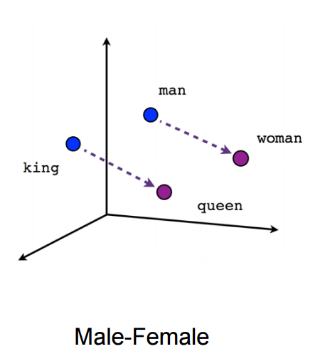
\includegraphics[scale=0.4]{images/embeddings.png}
    \end{center}
\end{frame}

\begin{frame}

\frametitle{What is language model?}

A \textbf{language model} is a probability distribution over sequences of words. It assigns a probability for a sequence of words

$$
    P(w_1, \cdots. w_{n})
$$

\textbf{Neural net language models}

Learn to predict next word in the sequence based on the context
$$
P(w_{i}|{\mathrm  {context}})
$$

\end{frame}

\begin{frame}
    \frametitle{Modern approaches to NLP tasks}
    \begin{itemize}
        \item RNN (Recurrent neural network) (vanishing gradient problem)
        \item LSTM (Long short-term memory) \parencite{hochreiter1997long} (capture longer context)
        \item Bi-LSTM (process context in both directions)
        \item Transformers (drop LSTM $\to$ attention \parencite{vaswani2017attention})
    \end{itemize}
\end{frame}

\begin{frame}
    \frametitle{Transformer approach}
    \begin{itemize}
        \item attention seeing entire sequence as a whole
        \item much easier to train in paralell
        \item unsupervised pretraining then transfer learning
        \item text classification, question answering, machine translation etc.
        \item GPT, BERT, GPT-2, XLNet, Megatron, Turing-NLG
    \end{itemize}

    \begin{figure}[hbt!]
    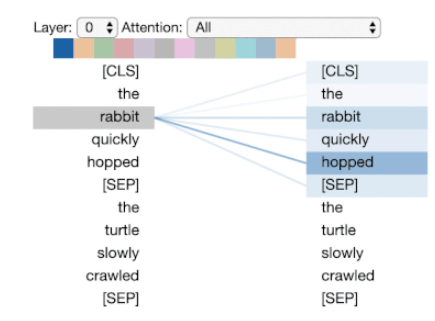
\includegraphics[scale=0.3]{images/attention.png}
    \caption{https://github.com/jessevig/bertviz}
    \end{figure}
\end{frame}

\section[Section]{BERT}

\begin{frame}
    \frametitle{What is BERT?}
    \begin{itemize}
        \item Bidirectional Encoder Representations from Transformers \parencite{devlin2018bert}
        \item method of pretraining language representation
        \item transformer based architecture (with slight differences)
        \item WordPiece embeddings
        \item you can fine-tune such model on a specific task
        \item classification, named-entity recognition, question answering etc.
        \item state of the art results on a number of NLP tasks at that time
    \end{itemize}
\end{frame}

\begin{frame}
    \frametitle{BERT Tokenizer}
    \begin{itemize}
        \item WordPiece embeddings (subword tokenization)\parencite{wordPiece}
        \item BERT input is constrained to 512 tokens
        \item special tokens [CLS], [SEP], [PAD] tokens
        \item positional embeddings, segment embeddings, token embeddings
    \end{itemize}
    \begin{figure}
    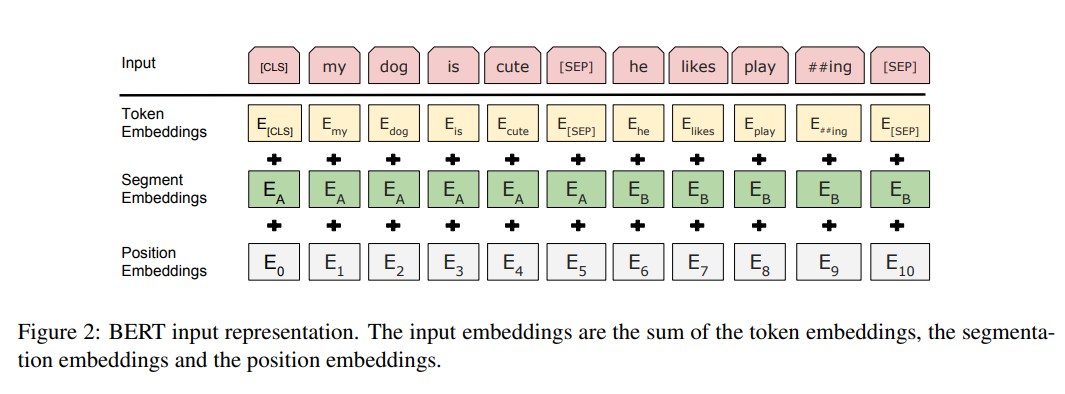
\includegraphics[scale=0.3]{images/bert_internal_representation.png}
    \end{figure}
\end{frame}

\begin{frame}
    \frametitle{Pretraining (BERT)}    
    \begin{itemize} 
        \item BooksCorpus (800m words), English Wikipedia (2500M words)
        \item masked language modelling (MLM), next sentence prediction (NSP)
        \item pretraining is expensive, load already pretrained models - BERT (base), BERT (large)
        \item leverage transfer learning by pretraining just once and then fine-tune on specific tasks
    \end{itemize}
    \begin{figure}
        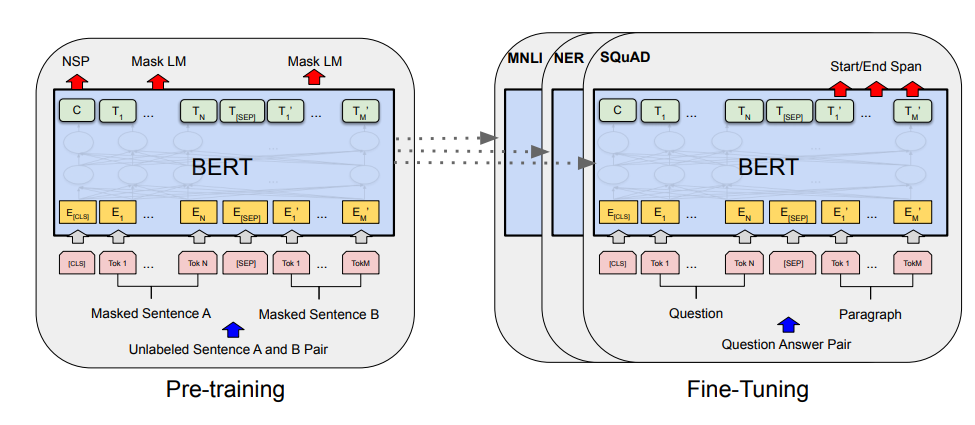
\includegraphics[scale=0.25]{images/pretraining.png}
    \end{figure}

\end{frame}


\begin{frame}
    \frametitle{BERT fine-tunning}
    Load the pretrained model and add task specific layer
    \begin{figure}
        % Your image included here
    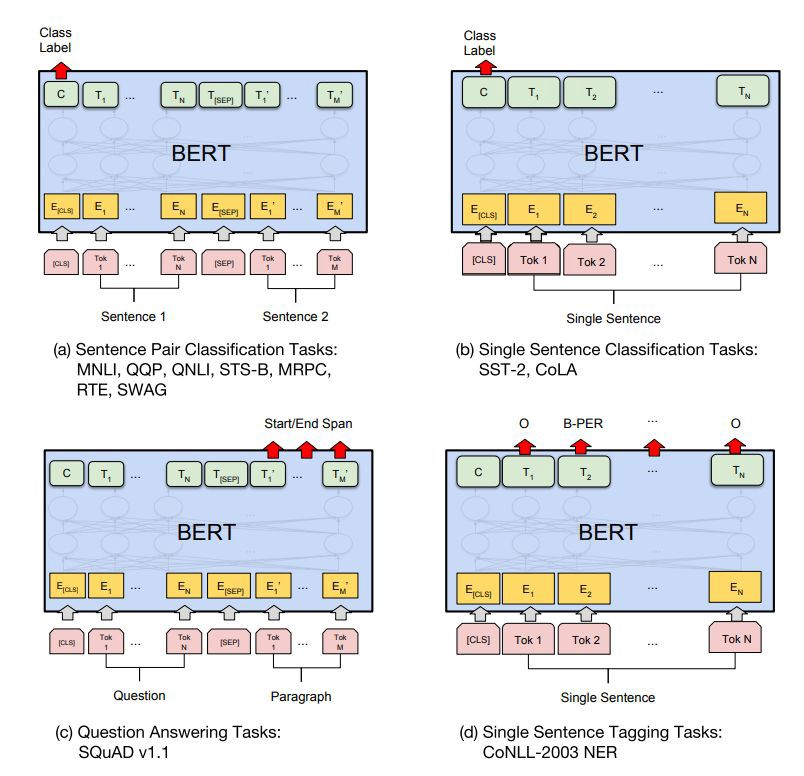
\includegraphics[scale=0.24]{images/fine-tunning.jpeg}
    \end{figure}
\end{frame}

%------------------------------------------------

\section{Practical Part}

\begin{frame}
    \frametitle{IMDB examples}
    
    \begin{table}
    \begin{tabular}{p{8cm} l}
    \toprule
    \textbf{Review} & \textbf{Sentiment} \\
    \midrule
    Probably my all-time favorite movie, a story of selflessness, sacrifice and dedication to a noble cause, & Positive  \\
    \midrule
    Encouraged by the positive comments about this film on here I was looking forward to watching this film. Bad mistake. I've seen 950+ films and this is truly one of the worst of them...  & Negative  \\
    \bottomrule
    \end{tabular}
    \caption{Examples in IMDB dataset}
    \end{table}
\end{frame}
\begin{frame}
    \frametitle{State of the art results on IMDB dataset}
    
    \begin{table}
    \begin{tabular}{l l p{5cm}}
    \toprule
    \textbf{Model} & \textbf{Accuracy} & \textbf{Paper/Source}\\
    \midrule
    XLNet & 96.21 & \parencite{yang2019xlnet} \\
    $BERT_{large} ITPT-FiT$ & 95.79 & \parencite{sun2019finetune} \\
    $BERT_{base} ITPT-FiT$ & 95.63 & \parencite{sun2019finetune} \\
    ULMFiT & 95.4 &  \parencite{howard2018universal} \\ 
    Block-sparse LSTM & 94.99 & \parencite{Gray2017GPUKF} \\ 
    \bottomrule
    \end{tabular}
    \caption{Performance on IMDB review dataset (\href{http://nlpprogress.com/english/sentiment_analysis.html}{nlpprogress.com})}
    \end{table}
\end{frame}

\begin{frame}
    \frametitle{IMDB sentiment analysis with BERT (practical part)}
    \begin{itemize}
        \item installation (we will use Google Colab)
        \item load IMDB using TensorFlow datasets
        \item BERT tokenizer
        \item load pretrained BERT model (transformers library)
        \item compile model choose loss, optimizer etc.
        \item fine-tunning the model
        \item evaluate the model
    \end{itemize}

    \begin{figure}
        % Your image included here
    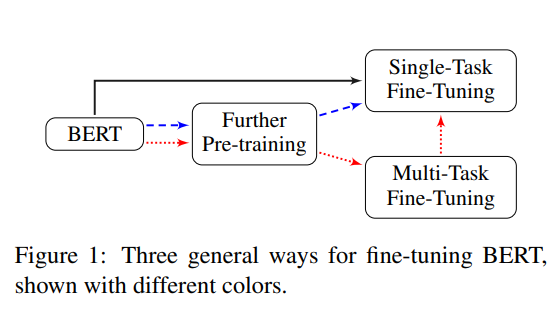
\includegraphics[scale=0.28]{images/fine-tunning-strategies.png}
    \end{figure}

\end{frame}

%------------------------------------------------


\begin{frame}

\Huge\centerline{\href{
    https://colab.research.google.com/drive/1934Mm2cwSSfT5bvi78-AExAl-hSfxCbq}{Google Colab}
}

\end{frame}



\begin{frame}[allowframebreaks]
\frametitle{References}
    \printbibliography
\end{frame}

%----------------------------------------------------------------------------------------

\end{document} 

